% !TEX root = ../0_tcc.tex

\begin{figure}[ht]
	\centering
		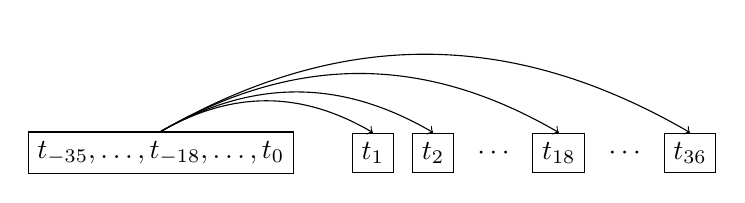
\begin{tikzpicture}
			\node[draw, rectangle]  at  (0,0)  (ts-36)
			{$t_{-35}, \dots, t_{-18}, \dots, t_{0} $};

			\node[draw, rectangle] at ([xshift=1cm]ts-36.east)   (ts1)   {$t_1$};
			\draw[->]  (ts-36.north) [bend left] to (ts1.north)  ;

			\node[draw, rectangle] at ([xshift=0.5cm]ts1.east)   (ts2)   {$t_2$};
			\draw[->]  (ts-36.north) [bend left] to (ts2.north)  ;

			\node[] at ([xshift=0.5cm]ts2.east)   (tsdot) {$\cdots$};

			\node[draw, rectangle] at ([xshift=0.5cm]tsdot.east) (ts18)  {$t_{18}$};
			\draw[->]  (ts-36.north) [bend left] to (ts18.north)  ;

			\node[] at ([xshift=0.5cm]ts18.east)   (tsdot2) {$\cdots$};

			\node[draw, rectangle] at ([xshift=0.5cm]tsdot2.east)  (ts36)  {$t_{36}$};
			\draw[->]  (ts-36.north) [bend left] to (ts36.north)  ;
		\end{tikzpicture}
	\caption{Esquema de várias redes para previsão individual de timesteps. Fonte: própria.}\label{tikz:nns}
\end{figure}
